% ==========================================
% CHAPTER 3: FLUID DYNAMICS
% ==========================================
\section{Fluid Dynamics \& Streamline Analysis}

\subsection{The Bernoulli Equation}

Applying Newton's Second Law ($\Sigma \vec{F} = m\vec{a}$) along a streamline (s-direction):
\begin{equation*}
    -\frac{\partial P}{\partial s} - \rho g \frac{\partial z}{\partial s} = \rho v \frac{\partial v}{\partial s}
\end{equation*}

Integrating along the streamline with constant $\rho$ gives the \textbf{Bernoulli Equation (1738)}:
\begin{eqbox}{Bernoulli's Equation}
\begin{equation}
    P + \frac{1}{2}\rho v^2 + \rho g z = \text{Constant}
\end{equation}
\textbf{Strict Assumptions:} 1) Steady flow, 2) Incompressible fluid ($\rho = cst$), 3) Inviscid flow (no friction/shear), 4) Along a single streamline.
\end{eqbox}

\subsubsection{Stagnation Point}

When fluid hits a blunt object, the streamline dividing the flow stops completely at the \textbf{Stagnation Point (SP)} where $v = 0$.

\vspace{0.3cm}
\begin{center}
\begin{tikzpicture}[scale=1.2, >=Stealth]
    % Object (gray wedge with curved nose)
    \filldraw[fill=gray!30, draw=black, thick] 
        (1.5, 1.5) arc(180:120:1) -- (4, 3) -- (4, 0) -- (1.0, 0.634) arc(240:180:1) -- cycle;
        
    % Streamlines
    \draw[thick, primary, ->] (-1, 2) .. controls (0.5, 2) and (1, 2.5) .. (3, 2.8);
    \draw[thick, primary, ->] (-1, 2.5) .. controls (0.5, 2.5) and (1, 3.2) .. (3, 3.5);
    \draw[thick, primary, ->] (-1, 1) .. controls (0.5, 1) and (1, 0.5) .. (3, 0.2);
    \draw[thick, primary, ->] (-1, 0.5) .. controls (0.5, 0.5) and (1, -0.2) .. (3, -0.5);
    
    % Central streamline
    \draw[thick, primary] (-1, 1.5) -- (0, 1.5);
    \draw[thick, primary, ->] (0, 1.5) -- (0.8, 1.5);
    \draw[thick, primary, dashed] (0.8, 1.5) -- (1.5, 1.5);
    
    % Points
    \filldraw[black] (-0.2, 1.5) circle (1.5pt) node[above] {1 ($P_1, v_1$)};
    \filldraw[accent] (1.5, 1.5) circle (2.5pt) node[right, black] {SP ($v_2 = 0$)};
\end{tikzpicture}
\end{center}
\vspace{0.3cm}

Using Bernoulli from point 1 to the Stagnation Point (point 2):
\begin{equation*}
    P_1 + \frac{1}{2}\rho v_1^2 = P_2 + 0 \implies P_2 = P_1 + \frac{1}{2}\rho v_1^2 = P_{\text{stagnation}}
\end{equation*}

\subsubsection{Flow Across Streamlines}
In the normal direction ($n$) towards the center of curvature $R_n$:
\begin{equation*}
    -\frac{\partial P}{\partial n} - \rho g \frac{\partial z}{\partial n} = \rho \frac{v^2}{R_n}
\end{equation*}

Integrating this equation across the streamlines (along $dn$), we obtain the exact result:
\begin{equation*}
    P + \rho g z + \rho \int \frac{v^2}{R_n} \, dn = \text{Constant}
\end{equation*}
This mathematically shows that the pressure increases as one moves radially away from the center of curvature.

\subsection{Rectilinear Streamlines}

Consider rectilinear (or nearly rectilinear) streamlines. 
The radius of curvature $R \rightarrow \infty$.

\begin{center}
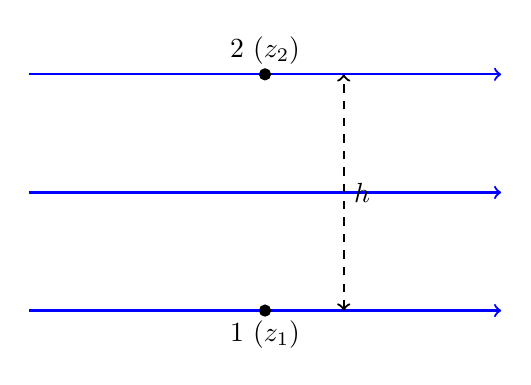
\begin{tikzpicture}
    % Streamlines
    \draw[->, thick, blue] (0, 0) -- (6, 0);
    \draw[->, thick, blue] (0, 1.5) -- (6, 1.5);
    \draw[->, thick, blue] (0, 3) -- (6, 3);
    
    % Points
    \filldraw[black] (3, 0) circle (2pt) node[below] {1 ($z_1$)};
    \filldraw[black] (3, 3) circle (2pt) node[above] {2 ($z_2$)};
    
    % Dimensions
    \draw[<->, dashed, thick] (4, 0) -- (4, 3) node[midway, right] {$h$};
\end{tikzpicture}
\end{center}

For the pressure difference between points 1 and 2, we apply the hydrostatic principles (first comprehensively detailed by Blaise Pascal in 1648):
\begin{align*}
    p_2 - p_1 &= -\rho g (z_2 - z_1) \\
    \tcbhighmath{p_1 = p_2 + \rho g h} \quad &\text{(hydrostatic result)}
\end{align*}

\subsection{Example: Pitot-Tube (Speed Sensor)}

\textbf{Task:} Determine velocity $v$.
The Pitot-tube was invented by French engineer Henri Pitot in 1732 to measure fluid flow velocity.

\begin{center}
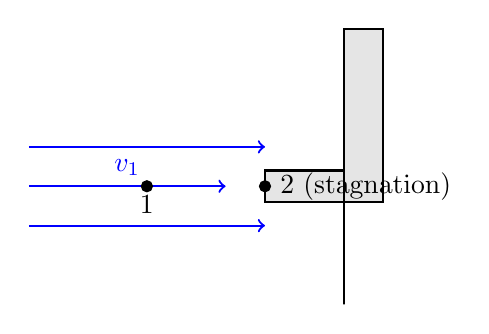
\begin{tikzpicture}
    % Flow
    \draw[->, thick, blue] (-2, 0) -- (0.5, 0) node[midway, above] {$v_1$};
    \draw[->, thick, blue] (-2, 0.5) -- (1, 0.5);
    \draw[->, thick, blue] (-2, -0.5) -- (1, -0.5);
    
    % Pitot Tube
    \draw[thick, fill=gray!20] (2, -1.5) -- (2, 2) -- (2.5, 2) -- (2.5, -0.2) -- (1, -0.2) -- (1, 0.2) -- (2, 0.2) -- cycle;
    
    % Points
    \filldraw[black] (-0.5, 0) circle (2pt) node[below] {1};
    \filldraw[black] (1, 0) circle (2pt) node[right, xshift=2pt] {2 (stagnation)};
    
\end{tikzpicture}
\end{center}

Along this streamline, the total pressure $p_t = \text{cte}$ (neglecting gravity). Applying Bernoulli's equation (published by Daniel Bernoulli in 1738) from point 1 to point 2:
\begin{equation*}
    p_1 + \frac{1}{2}\rho v_1^2 = p_2 + \frac{1}{2}\rho v_2^2
\end{equation*}
Since point 2 is a stagnation point, $v_2 = 0$:
\begin{align*}
    p_1 + \frac{1}{2}\rho v_1^2 &= p_2 + 0 \\
    p_2 - p_1 &= \frac{1}{2}\rho v_1^2
\end{align*}
Solving for the velocity $v_1$:
\begin{equation*}
    \tcbhighmath{v_1 = \sqrt{\frac{2(p_2 - p_1)}{\rho}}}
\end{equation*}

\subsection{Mass Conservation \& Stream Tubes}

Useful concept: Mass Conservation in a stream tube. The continuity equation for steady incompressible flow was first mathematically formulated by Benedetto Castelli in 1628.

\begin{center}
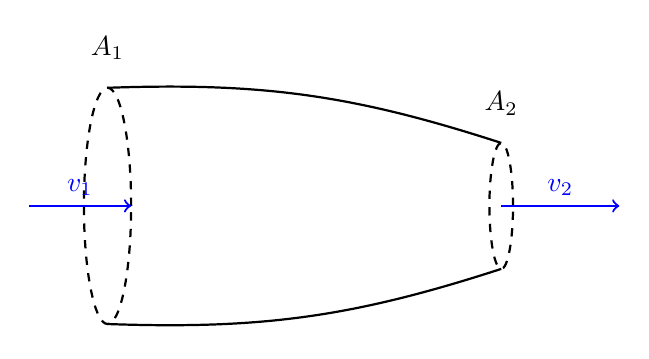
\begin{tikzpicture}
    % Stream tube walls
    \draw[thick] (0, 1.5) to[bend left=10] (5, 0.8);
    \draw[thick] (0, -1.5) to[bend right=10] (5, -0.8);
    
    % Cross sections
    \draw[dashed, thick] (0,0) ellipse (0.3 and 1.5);
    \draw[dashed, thick] (5,0) ellipse (0.15 and 0.8);
    
    % Flow vectors and labels
    \node at (0, 2) {$A_1$};
    \draw[->, thick, blue] (-1, 0) -- (0.3, 0) node[midway, above] {$v_1$};
    
    \node at (5, 1.3) {$A_2$};
    \draw[->, thick, blue] (5, 0) -- (6.5, 0) node[midway, above] {$v_2$};
\end{tikzpicture}
\end{center}

\begin{itemize}
    \item Mass flow rate: $\dot{m} \quad \left[ \frac{\text{kg}}{\text{s}} \right]$
    \item Volume flow rate: $\dot{V} \quad \left[ \frac{\text{m}^3}{\text{s}} \right]$
\end{itemize}
\begin{equation*}
    \dot{V} = v A \quad \text{(velocity $\times$ area)}
\end{equation*}
Conservation of mass principle:
\begin{equation*}
    \rho_1 v_1 A_1 = \rho_2 v_2 A_2
\end{equation*}
Assuming steady and incompressible flow ($\rho_1 = \rho_2$):
\begin{equation*}
    \tcbhighmath{v_1 A_1 = v_2 A_2}
\end{equation*}

\subsection{Example: Venturi Meter}

Invented by Italian physicist Giovanni Battista Venturi in 1797, this device measures flow rate by reducing the cross-sectional area of flow.

\begin{center}
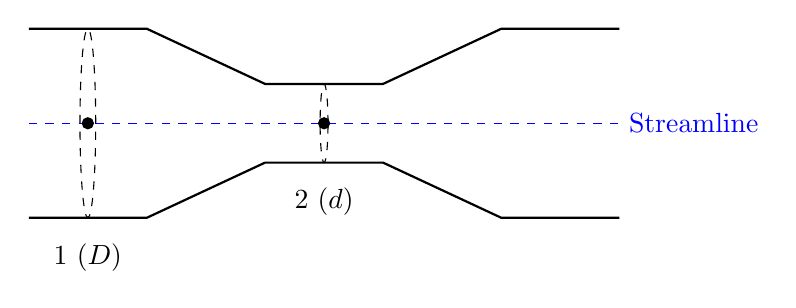
\begin{tikzpicture}
    % Pipe shape
    \draw[thick] (0, 1.2) -- (1.5, 1.2) -- (3, 0.5) -- (4.5, 0.5) -- (6, 1.2) -- (7.5, 1.2);
    \draw[thick] (0, -1.2) -- (1.5, -1.2) -- (3, -0.5) -- (4.5, -0.5) -- (6, -1.2) -- (7.5, -1.2);
    
    % Streamline
    \draw[dashed, blue] (0,0) -- (7.5,0) node[right] {Streamline};
    
    % Points
    \draw[dashed] (0.75, 0) ellipse (0.1 and 1.2) node[below=1.4cm] {1 ($D$)};
    \draw[dashed] (3.75, 0) ellipse (0.05 and 0.5) node[below=0.7cm] {2 ($d$)};
    
    \filldraw[black] (0.75, 0) circle (2pt);
    \filldraw[black] (3.75, 0) circle (2pt);
\end{tikzpicture}
\end{center}

\textbf{Q: Flow rate?}

Apply Bernoulli's equation between points 1 and 2:
\begin{equation*}
    \frac{1}{2}\rho v_1^2 + p_1 + \rho g z_1 = \frac{1}{2}\rho v_2^2 + p_2 + \rho g z_2
\end{equation*}
Assuming horizontal flow ($z_1 = z_2$), the elevation terms cancel out:
\begin{equation*}
    v_1^2 + \frac{2(p_1 - p_2)}{\rho} = v_2^2
\end{equation*}
This leaves us with 2 unknowns ($v_1$ and $v_2$). We use Volume Conservation to find the second relationship:
\begin{equation*}
    v_1 A_1 = v_2 A_2 \implies v_1 D^2 = v_2 d^2 \implies v_2 = v_1 \left(\frac{D}{d}\right)^2
\end{equation*}
Substitute $v_2$ back into the simplified Bernoulli equation to solve for $v_1$:
\begin{equation*}
    \tcbhighmath{v_1 = \sqrt{ \frac{2(p_1 - p_2)}{\rho \left[ \left(\frac{D}{d}\right)^4 - 1 \right]} }}
\end{equation*}

\subsection{Example: Free Jet}

This scenario demonstrates Torricelli's Law, discovered experimentally by Evangelista Torricelli in 1643. We consider a bath (tank) with a tube/outlet at the bottom where water flows vertically downward.

\begin{center}
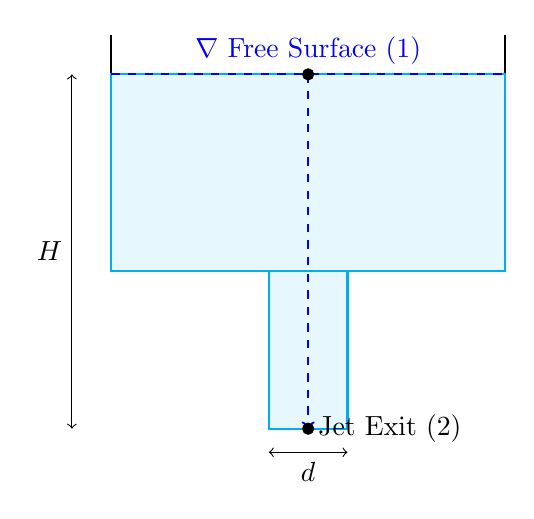
\begin{tikzpicture}
    % Bath (Tank)
    \draw[thick] (0, 3) -- (0, 0) -- (2, 0);
    \draw[thick] (3, 0) -- (5, 0) -- (5, 3);
    
    % Tube at bottom
    \draw[thick] (2, 0) -- (2, -2);
    \draw[thick] (3, 0) -- (3, -2);
    
    % Water inside the tank and tube
    \draw[thick, cyan, fill=cyan!10] (0, 0) rectangle (5, 2.5);
    \draw[thick, cyan, fill=cyan!10] (2, 0) rectangle (3, -2);
    
    % Free surface
    \draw[thick, blue, dashed] (0, 2.5) -- (5, 2.5);
    \node[blue] at (2.5, 2.8) {$\nabla$ Free Surface (1)};
    
    % Streamline
    \draw[->, thick, dashed, blue] (2.5, 2.5) -- (2.5, -2) node[right, black] {Jet Exit (2)};
    
    % Points
    \filldraw[black] (2.5, 2.5) circle (2pt);
    \filldraw[black] (2.5, -2) circle (2pt);
    
    % Dimensions
    \draw[<->] (-0.5, -2) -- (-0.5, 2.5) node[midway, left] {$H$};
    \draw[<->] (2, -2.3) -- (3, -2.3) node[midway, below] {$d$};
\end{tikzpicture}
\end{center}

\textbf{Assumptions:}
\begin{itemize}
    \item No shear forces
    \item $\rho = \text{const}$ (in incompressible)
    \item Steady or quasi-steady flow evaluated along a streamline
\end{itemize}

Applying Bernoulli's equation from the free surface (1) to the exiting jet (2):
\begin{equation*}
    \frac{1}{2}\rho v_1^2 + \rho g z_1 + p_1 = \frac{1}{2}\rho v_2^2 + \rho g z_2 + p_2
\end{equation*}
We define the conditions:
\begin{itemize}
    \item $v_1 \approx 0$ (large tank assumption)
    \item $z_1 - z_2 = H$ (total height difference to the tube exit)
    \item $p_1 = p_2 = p_{\text{atm}}$
\end{itemize}
Simplifying the equation gives Torricelli's result:
\begin{align*}
    \rho g H &= \frac{1}{2}\rho v_2^2 \\
    \tcbhighmath{v_2 = \sqrt{2gH}}
\end{align*}

The flow rate out of the tube is determined by the velocity and the area of the jet:
\begin{equation*}
    \tcbhighmath{\dot{V} = v_2 A_2 = \sqrt{2gH} \left(\frac{\pi}{4} d^2\right)}
\end{equation*}

\subsection{Vena Contracta}

Independent of the bottom-tube free jet, the \textit{vena contracta} effect occurs when fluid flows through a sharp-edged orifice (a phenomenon first properly identified and measured by Isaac Newton in the second edition of his Principia in 1713). The streamlines cannot abruptly change direction, causing the exiting jet to contract to a diameter smaller than the physical hole.

\begin{center}
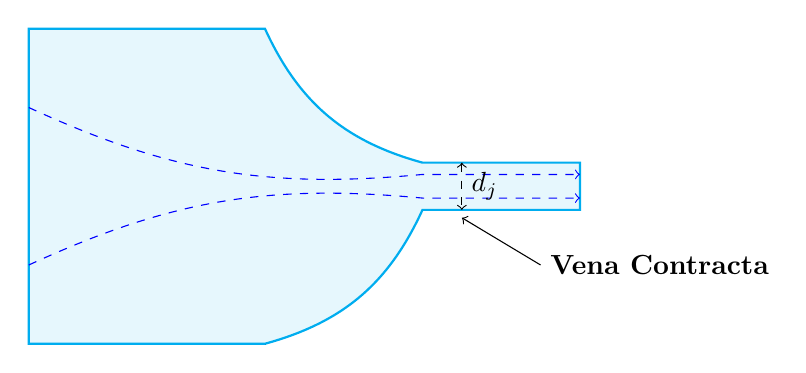
\begin{tikzpicture}
    % Tank walls (sharp edged)
    \draw[thick, fill=gray!30] (0, 2) -- (0, 0.5) -- (-0.5, 0.5) -- (-0.5, 2) -- cycle;
    \draw[thick, fill=gray!30] (0, -2) -- (0, -0.5) -- (-0.5, -0.5) -- (-0.5, -2) -- cycle;
    
    % hole diameter
    \draw[<->, dashed] (0.2, 0.5) -- (0.2, -0.5) node[midway, right] {$d_h$};
    
    % Fluid and Streamlines
    \draw[thick, cyan, fill=cyan!10] (-3, 2) -- (0, 2) to[bend right=25] (2, 0.3) -- (4, 0.3) -- (4, -0.3) -- (2, -0.3) to[bend left=25] (0, -2) -- (-3, -2) -- cycle;
    
    % Streamline lines
    \draw[->, blue, dashed] (-3, 1) to[bend right=15] (2, 0.15) -- (4, 0.15);
    \draw[->, blue, dashed] (-3, -1) to[bend left=15] (2, -0.15) -- (4, -0.15);
    
    % jet diameter
    \draw[<->, dashed] (2.5, 0.3) -- (2.5, -0.3) node[midway, right] {$d_j$};
    
    % Vena Contracta label
    \draw[<-] (2.5, -0.4) -- (3.5, -1) node[right] {\textbf{Vena Contracta}};
\end{tikzpicture}
\end{center}

Because the streamlines converge as they exit the hole, the actual jet area ($A_j$) is smaller than the hole area ($A_h$). The contraction coefficient $C_c$ is defined as:
\begin{equation*}
    \tcbhighmath{C_c = \frac{A_j}{A_h} = \left(\frac{d_j}{d_h}\right)^2}
\end{equation*}